%% LaTeX-Beamer template for KIT design
%% by Erik Burger, Christian Hammer
%% title picture by Klaus Krogmann
%%
%% version 2.1
%%
%% mostly compatible to KIT corporate design v2.0
%% http://intranet.kit.edu/gestaltungsrichtlinien.php
%%
%% Problems, bugs and comments to
%% burger@kit.edu

\documentclass[18pt]{beamer}
\usepackage[utf8x]{inputenc}
\usepackage{units}
\usepackage{booktabs}

%% CUSTOM
\usepackage{amsmath}
\usepackage{algpseudocode}

%% Definitions
\DeclareMathOperator{\div2}{div}
\renewcommand{\algorithmicrequire}{\textbf{Input:}}
\renewcommand{\algorithmicensure}{\textbf{Output:}}
\algnewcommand\algorithmicto{\textbf{to}}
\algrenewtext{For}[3]{\algorithmicfor\ $#1 \gets #2$ \algorithmicto\ $#3$ \algorithmicdo}
\algnewcommand\algorithmicod{\textbf{od}}
\algrenewtext{EndWhile}{\algorithmicod}
\algrenewtext{EndFor}{\algorithmicod}
%\AtBeginSection[]{%
%\begin{frame}<beamer> % do nothing in handouts
%    \frametitle{Überblick}
%    \tableofcontents[sectionstyle=show/shaded,
%    subsectionstyle=show/show/hide]
%\end{frame}
%}
%\AtBeginSubsection[]{%
%\begin{frame}<beamer> % do nothing in handouts
%    \frametitle{Überblick}
%    \tableofcontents[sectionstyle=show/shaded,
%    subsectionstyle=show/shaded/hide]
%\end{frame}
%}

%% SLIDE FORMAT

% use 'beamerthemekit' for standard 4:3 ratio
% for widescreen slides (16:9), use 'beamerthemekitwide'

\usepackage{templates/beamerthemekit}
%\usepackage{templates/beamerthemekitwide}

 %% TITLE PICTURE

 % if a custom picture is to be used on the title page, copy it into the 'logos'
 % directory, in the line below, replace 'mypicture' with the 
 % filename (without extension) and uncomment the following line
 % (picture proportions: 63 : 20 for standard, 169 : 40 for wide
 % *.eps format if you use latex+dvips+ps2pdf, 
 % *.jpg/*.png/*.pdf if you use pdflatex)


 \titleimage{banner}
 
 
%% Define some colors:
\definecolor{darkblue}{rgb}{0,0,.5}
\definecolor{darkgreen}{rgb}{0,.5,0}

 %% TITLE LOGO

 % for a custom logo on the front page, copy your file into the 'logos'
 % directory, insert the filename in the line below and uncomment it

\titlelogo{logo_150x150}
 
 % (*.eps format if you use latex+dvips+ps2pdf,
 % *.jpg/*.png/*.pdf if you use pdflatex)
 
 %% TikZ INTEGRATION
 
 % use these packages for PCM symbols and UML classes
 % \usepackage{templates/tikzkit}
 % \usepackage{templates/tikzuml}
 
 % the presentation starts here
 
\author{Dominik Muth - dominik.muth@student.kit.edu}
\institute{Institut f\"ur Informatik}


\title[Tutorium 10]{GBI Tutorium Nr. $2^5$}
\subtitle{Tutorium 10}
\date{9. Januar 2013}

% Bibliography



\begin{document}

	%title page
	\begin{frame}
		\titlepage
	\end{frame}

	%table of contents
	\begin{frame}{Outline/Gliederung}
		\tableofcontents
	\end{frame}	
		
	
	
	\section{Wiederholung} 
	\begin{frame} {Wiederholung - Quiz}
		\begin{itemize}
			\item Aus $f\in \Omega(g) \land f \in \Theta(g) \Rightarrow f \in \mathcal{O}(g)$
			\only<2-> {\color{darkgreen}$\surd$}\\
			\color{black}
					
			\item $n^5 \in \mathcal{O}(2^n)$
			\only<3-> {\color{darkgreen}$\surd$}\\
			\color{black}
	
			\item $\frac{n^3+2n}{2n+1} \in \mathcal{O}(n)$
			\only<4-> {\color{red}$X$}\\
			\color{black}
			
			\item Alle Algorithmen liegen in $\Omega(1)$
			\only<5-> {\color{darkgreen}$\surd$}\\
			\color{black}
		\end{itemize}
	\end{frame}
	
	
	
	\section{Master Theorem}
	\begin{frame}{Master Theorem}
		\begin{block}{Wozu?}
			Laufzeitabschätzung von rekursiv definierten Funktionen
		\end{block}
		
		\pause
		\begin{block}{Grundaufbau}
			\[T(n) = a\cdot T(\frac{n}{b}) + f(n)\]
		\end{block}
		
		\pause
		\begin{block}{Erläuterung}
			\begin{itemize}
				\item $a$ = Anzahl der Unterprobleme in der Rekursion
				
				\pause
				\item $\frac{1}{b}$ = Teil des Originalproblems, welches wiederum durch alle Unterprobleme repräsentiert wird
				
				\pause
				\item $f(n)$ = Aufwand, welcher durch die Rekursion der Teilprobleme und Kombination der Teillösungen auftritt.
			\end{itemize}
		\end{block}
	\end{frame}
	
	
	\begin{frame}{Master Theorem}
		\begin{block}{Wie funktionierts?}
			Man unterscheidet zwischen 3 Fällen:
			\begin{enumerate}
				\pause
				\item Wenn $f(n) \in \mathcal{O}(n^{log_b a-\epsilon})$ mit $\epsilon > 0$, $\Rightarrow T(n) \in \Theta(n^{log_b a})$
				\vspace{10pt}
				
				\pause
				\item Wenn $f(n) \in \Theta(n^{log_b a}$, $\Rightarrow T(n) \in \Theta(n^{log_b a}log n)$
				\vspace{10pt}
				
				\pause
				\item Wenn $f(n) \in \Omega(n^{log_b a+\epsilon}$ mit $\epsilon > 0$, \\
				und wenn es ein $c$ gibt, mit $ 0 < c < 1$, \\
				sodass für alle hinreichend großen n gilt: $a\cdot f(\frac{n}{b}) \leq c \cdot f(n)$,\\
				$\Rightarrow T(n) \in \Theta(f(n))$
			\end{enumerate}
		\end{block}
	\end{frame}
	
	\begin{frame}{Master Theorem}
		\begin{exampleblock}{Beispiele}
			\[49 \cdot T( \frac{n}{7} ) + 3n + 5\]\\
			\[49 \cdot T( \frac{n}{7} ) + 3n^3 + 5\]\\
		\end{exampleblock}
	\end{frame}
	
	
	
	\section{Mealy-Automaten}
	\begin{frame}{Mealy-Automaten}
		\begin{block}{Definition: Mealy-Automat}
        Der Mealy-Automat $A = \left( Z, z_0, X, f, Y, g \right)$ besteht aus
        	\begin{itemize}
            	\item der endlichen Zustandsmenge $\mathbf{Z}$,
				\pause
            	\item dem Startzustand $\mathbf{z_0}$,
				\pause
            	\item dem Eingabealphabet $\mathbf{X}$,
				\pause
            	\item der Zustandsübergangsfunktion $\mathbf{f: Z\times X \rightarrow Z}$,
				\pause
            	\item einem Ausgabealphabet $\mathbf{Y}$ und
				\pause
            	\item der Ausgabefunktion $\mathbf{g: Z\times X \rightarrow Y^*}$.
        	\end{itemize}
    	\end{block}
	\end{frame}
	
	
	\begin{frame}{Mealy-Automaten}
		\begin{block}{Interaktive Aufgabe}
			Einen Getränke$\mathbf{automaten}$ modellieren:\\
			saurer Sprudel = $rein$ (Eingabe/Ausgabe: R)\\
			süßer Sprudel = $zitro$ (Eingabe/Ausgabe: Z)\\
			Abbrechen = $C$ (Eingabe: C)\\
			Bestätigen = $OK$ (Eingabe: O)\\
			Ein Getränk kostet 1 Euro (Eingabe: 1)
		\end{block}
		\begin{center}
		
		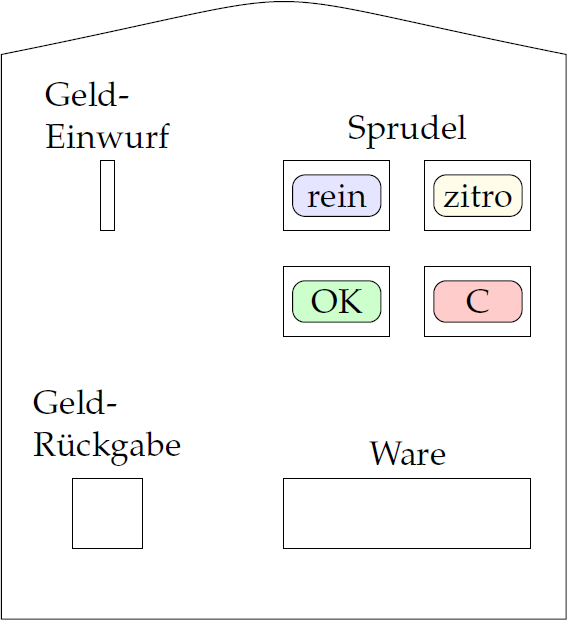
\includegraphics[scale=0.2]{graphics/10/getraenke.png}
		\end{center}
	\end{frame}
	
	
	\begin{frame}{Mealy-Automaten}
		\begin{block}{$f^*$ und $f^{**}$}
			$\mathbf{f^*}$: $f^*(z,w)$ kann im Gegensatz zu $f$ ein ganzes Wort $w$, als zweites Funktionsargument nehmen, und gibt somit an, in welchem Zustand sich man sich befindet, nachdem man das Wort $w$ abgearbeitet hat.\\
			\vspace{10pt}
			$\mathbf{f^{**}}$: $f^{**}(z,w)$ gibt die Durchlaufenen Zustände bei der Eingabe $w$ an.
		\end{block}
		
		\pause
		\begin{block}{$g^*$ und $g^{**}$}
			Simultan zu $f^*$ und $f^{**}$ geben die Funktionen $g^*(z,w)$ und $g^{**}(z,w)$ die Ausgabe nach dem eingegebenen Wort $w$ an.
		\end{block}
	\end{frame}
	
	
	\begin{frame}{Mealy-Automaten - Aufgaben}
		\begin{itemize}
			\item Berechnen Sie $f^{**}((0,-), RZR11C)$ für den an der Tafel stehenden Automaten
			\item Berechnen Sie $g^{**}((0,-), RZR11O)$ für den an der Tafel stehenden Automaten
		\end{itemize}
	\end{frame}
	
	
	
	\section{Moore-Automaten}
	\begin{frame}{Moore-Automaten}
		\begin{block}{Definition: Moore-Automat}
        Der Moore-Automat $A = \left( Z, z_0, X, f, Y, h \right)$ besteht aus
        	\begin{itemize}
            	\item der endlichen Zustandsmenge $\mathbf{Z}$,
				\pause
            	\item dem Startzustand $\mathbf{z_0}$,
				\pause
            	\item dem Eingabealphabet $\mathbf{X}$,
				\pause
            	\item der Zustandsübergangsfunktion $\mathbf{f: Z\times X \rightarrow Z}$,
				\pause
            	\item einem Ausgabealphabet $\mathbf{Y}$ und
				\pause
            	\item der Ausgabefunktion $\mathbf{h: Z \rightarrow Y^*}$.
        	\end{itemize}
        \end{block}
	\end{frame}
	
	
	\begin{frame}{Moore-Automaten}
		\begin{exampleblock}{Beispiel}
			\begin{center}
				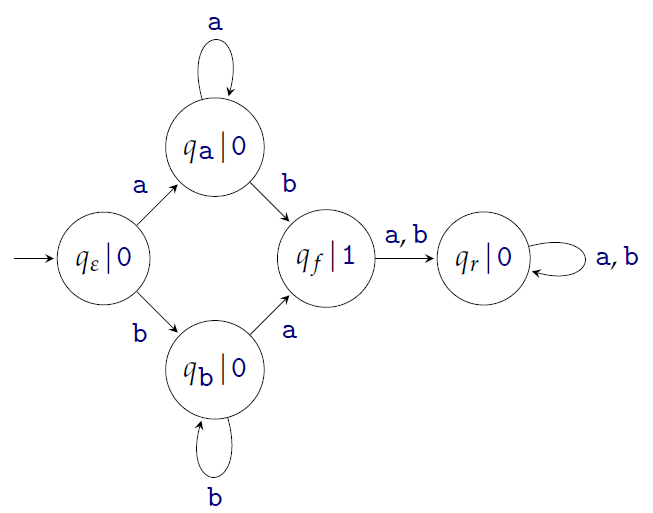
\includegraphics[scale=0.5]{graphics/10/moore.png}
			\end{center}
		\end{exampleblock}
	\end{frame}
	
	
	\begin{frame}{Moore-Automaten - Aufgaben}
		\begin{itemize}
			\item Wandeln Sie den Automaten von Eben in einen Mealy-Automaten um
			\item Modellieren Sie einen Automaten, welcher bei Wörter mit gerader Länge, welche mindestens einmal aa und einmal bb enthalten eine 1 ausgibt, sonst 0.
		\end{itemize}
	\end{frame}

		
	\section{Endliche Akzeptoren}
	\begin{frame}{Endliche Akzeptoren}
		\begin{block}{Definition}
			Ein endlicher Akzeptor $A = (Z, z_0, X, f , F)$ ist festgelegt durch:\\
			\begin{itemize}
				\pause
				\item eine endliche Zustandsmenge $\mathbf{Z}$,
				\pause
				\item einen Anfangszustand $\mathbf{z_0 \in Z}$,
				\pause
				\item ein Eingabealphabet $\mathbf{X}$,
				\pause
				\item eine Zustandsübergangsfunktion $\mathbf{f: Z\times X \rightarrow Z}$ und
				\pause
				\item eine Menge $\mathbf{F \subseteq Z}$ akzeptierender Zustände.
			\end{itemize}
			Akzeptierende Zustände werden in der Regel als doppelte Kringel dargestellt.
		\end{block}
	\end{frame}		
	
	
	\begin{frame}{Endliche Akzeptoren}
		\begin{exampleblock}{Beispiel}
			Ein endlicher Akzeptor, welcher alle Wörter aus $\{a,b\}^*$ akzeptiert, welche mit a anfangen und aufhören oder mit b anfangen und aufhören.
		\end{exampleblock}
	\end{frame}
	
	
	\begin{frame}{Endliche Akzeptoren - Aufgaben}
		\begin{itemize}
			\item Entwerfen Sie einen endlichen Akzeptor, mit $X=\{a,b\}$, der alle Wörter akzeptiert, bei denen die Anzahl der $a$ durch 5 teilbar ist.
			\item Entwerfen Sie einen endlichen Akzeptor, mit $X=\{a,b\}$, der alleWörter akzeptiert, in denen nirgends hintereinander zwei b vorkommen.
		\end{itemize}
	\end{frame}
	
	
	
	\section{Fragen}
	\begin{frame} {Fragen}
		\begin{itemize}
			\item Fragen zum Stoff?
			\item Fragen zum n\"achsten \"Ubungsblatt?
			\item Generelle Fragen?
			\item Feedback?
		\end{itemize}
	\end{frame}	
		
		
	\begin{frame} {Frohe Weihnachten}
		\begin{center}
			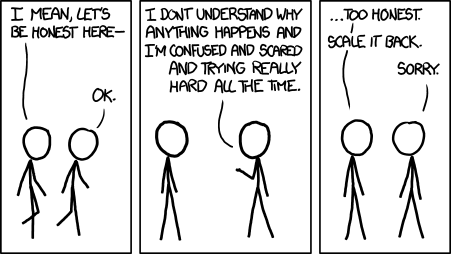
\includegraphics[scale=0.65]{graphics/eof10.png}\\
			\tiny $source: http://imgs.xkcd.com/comics/honest.png$
		\end{center}
	\end{frame}

\end{document}
